% \chapter{Базовые понятия и результаты}
\chapter{Обзор предметной области}
\label{ch:overview}

В данной главе представлены основные понятия и существующие результаты.


\section{Конечные автоматы}

Конечный автомат (КА) \--- это одна из простых моделей вычислений, свойствам которых посвящено огромное число работ. \todo{ссылки}
КА описывает систему с конечным числом состояний и переходов между ними.
Конечный автомат может быть задан в виде пятерки $\mathcal{A} = \Tuple{\Sigma, Q, q_0, F, \delta}$, где:
\begin{itemize}
    \item $\Sigma$ --- алфавит входных символов;
    \item $Q$ --- (\textit{конечное}) множество состояний;
    \item $q_0 \in Q$ --- начальное состояние;
    \item $F \subseteq Q$ --- множество терминальных (принимающих) состояний;
    \item $\delta \colon Q \times \Sigma \to Q$ --- функция переходов.
\end{itemize}
Конечный автомат \textit{принимает} (\textit{accepts}) слово $w = w_1 w_2 \ldots w_n \in \Sigma^*$, если после прочтения $w$ автомат оказывается в одном из терминальном состоянии $s_n \in F$, то есть существует последовательность состояний $s_0, s_1, \ldots, s_n$ такая, что $s_0 = q_0$, $s_{i+1} = \delta(s_i, w_{i+1})$ для всех $i \in \Set{0, 1, \ldots, n-1}$ и $s_n \in F$.

В настоящей работе исследуются задачи синтеза КА, обладающих определенными свойствами, а также задачи верификации уже построенных КА на предмет соответствия конкретным спецификациям~\cite{hachtel1996}.


\section{Булевы схемы}

% Булева схема может быть задана в виде кортежа $\mathcal{C} = \Tuple{I, O, G, L}$, где:
% \todo{пофиксить кортеж}
% \begin{itemize}
%     \item $I$ --- множество входных вершин (\textit{inputs});
%     \item $O$ --- множество выходных вершин (\textit{outputs});
%     \item $G$ --- множество внутренних вершин (\textit{gates});
% % \item $W \subseteq I \union G$ --- множество входных вершин, которые не являются входами схемы (\textit{wires});
%     \item $L \colon G \to \Set{\land, \lor, \neg, \dots}$ --- функция, которая каждой внутренней вершине сопоставляет логическую функцию.
% \end{itemize}

Булева схема \--- это направленный ациклический ориентированный граф $G = \Pair{V, E}$, где $V$ \=== множество вершин, а $E \subseteq V^2$ \=== множество рёбер (\textit{дуг}).
Вершины такого графа делятся на три типа: входные вершины (\textit{inputs}), выходные вершины (\textit{outputs}) и внутренние вершины (\textit{gates}).
\textit{Ребро} (\textit{дуга}) представляет собой упорядоченную пару вершин.
Для каждой дуги $(u,v) \in E$, вершина $u$ называется \textit{родителем}~$v$, а $v$ \=== \textit{потомком} $u$.
Множество всех родителей вершины~$v$ обозначается как~$P_v$.
Вершина называется \textit{входной}, если у нее нет родителей, и \textit{выходной}, если у нее нет потомков\footnote{Здесь стоит отметить, что вполне возможны вариации данных определений. В некоторых ситуациях \textit{входными}/\textit{выходными} вершинами в схеме считаются некоторые заранее выбранные вершины, но при этом у них могут быть родители/потомки, соотвественно. В зависимости от контекста, эти родители/потомки игнорируются в соответствующих определениях, связанных с обходом вершин графа от \textit{входов} к \textit{выходам}.}.
Множества входов и выходов обозначаются как $\Vin \subseteq V$ и $\Vout \subseteq V$ соответственно.
Любая вершина $v \in V \setminus \Vin$ называется \textit{гейтом} (\textit{логическим вентилем}).
В булевой схеме каждому гейту сопоставляется некоторый \textit{логический элемент} из предопределенного набора, называемого \textit{базисом} (например, $\{\land, \neg\}$).
Таким образом, любой логический элемент интерпретирует некоторую элементарную булеву функцию.
Пример булевой схемы представлен на Рисунке~\ref{fig:boolean-circuit-example}.

\begin{figure}[ht]
    \centering
    % \includegraphics[max width=0.5\textwidth]{example-image}
    \begin{adjustbox}{max width=\linewidth}
        \subfile{tex/tikz-circuit-example}
    \end{adjustbox}%
    \caption{Пример булевой схемы с тремя входами ($i_1$,~$i_2$,~$i_3$) и восьмью гейтами}
    \label{fig:boolean-circuit-example}
\end{figure}

Булева схема с $n$~входами и $m$~выходами естественным образом задает (тотальную) дискретную функцию $f \colon \{0, 1\}^n \to \{0, 1\}^m$, где под $\{0,1\}^k$ мы понимаем множество всех возможных двоичных слов длины~$k \in \Natural^{+}$.
Имея это в виду, мы будем использовать обозначение~$S_f$ для представления булевой схемы, задающей функцию~$f$.
Каждому гейту схемы $S_f$ сопоставлена булева функция, которая соответствует логическому элементу, назначенному этому гейту.

Пусть $\alpha\in\{0,1\}^n$ произвольное слово, поданное на вход~$S_f$.
Проходя по гейтам схемы в фиксированном порядке (обычно указанном топологической сортировкой~\cite{cormen1990}) и вычисляя значения элементарных функций, сопоставленных гейтам, мы получаем значение функции~$f$ на входном слове~$\alpha$ в качестве результата.
Этот процесс называется \textit{интерпретацией} схемы~$S_f$ на входе~$\alpha$.

Каждой вершине в схеме~$S_f$ сопоставим булеву переменную.
Обозначим множество переменных, ассоциированных с входами $\Vin$ схемы~$S_f$, как $\Xin = \{x_1,\dots,x_n\}$.
Переменные, связанные с гейтами, мы будем называть \textit{вспомогательными} (\textit{auxiliary}).
Пусть $u$ \=== некоторая вспомогательная переменная, соответствующая гейту~$v$, и $U_v$ \=== множество переменных, связанных с вершинами из~$P_v$.
Предположим, что $h_v$ \=== булева функция, соответствующая логическому элементу, назначенному гейту~$v$, и $F(h_v)$ \=== булева формула над~$U_v$, которая задает функцию~$h_v$.
Обозначим через $C_v$ КНФ-представление формулы $F(h_v) \equiv u$.

Рассмотрим следующую КНФ:
\begin{equation}\label{eq1}
    C_f = \biglandclap{v \in V \setminus \Vin} C_v
\end{equation}
Мы будем обозначать~\eqref{eq1} как \textit{шаблонную КНФ} для функции~$f$.
Заметим, что $C_f$~является КНФ-формулой, полученной применением преобразований Цейтина~\cite{tseitin1970} к схеме~$S_f$.

Ниже, следуя работе~\cite{szeider2006}, будем использовать обозначение~$x^{\sigma}$, где $\sigma \in \{0,1\}$, предполагая, что $x^0$ обозначает отрицательный литерал~$\neg x$, а $x^1$ обозначает положительный литерал~$x$, а также обозначение $\{0,1\}^{|B|}$, что означает множество всех возможных назначений переменных из~$B$.
%Пусть~$F$ будет произвольной булевой формулой над переменными~$X$.
%Обозначим через~$F|_{x=\sigma}$ формулу, полученную подстановкой~$x$ на место~$\sigma$ в~$F$~\cite{chang1973}.
%Очевидно, что формы $x^\sigma\land F$ и $F|_{x=\sigma}$ являются равноправными по удовлетворимости.
%Таким образом, когда мы работаем с формулой $x^\sigma \land F$, мы можем рассматривать единичную дизъюнкцию~$x^\sigma$ как значение~$\sigma$ переменной~$x$ в~$F$.
%Для произвольного набора булевых переменных~$B$ через $\{0,1\}^{|B|}$ мы обозначаем множество всех возможных назначений переменных из~$B$.
Следующий факт был многократно установлен в литературе, например, см.~\cite{bessiere2009,drechsler2009}.
Он использует простой механизм булевой дедукции, известный как правило распространения единичного дизъюнкта (Unit Propagation \--- UP)~\cite{marques-silva2009}.

\begin{lemma}\label{lem1}
    Применение UP к КНФ-формуле $x_1^{\alpha_1} \land \dots \land x_n^{\alpha_n} \land C_f$ для любого $\alpha = (\alpha_1, \dots, \alpha_n)$, $\alpha \in \{0,1\}^{|\Xin|}$ выводит (в форме единичных дизъюнкций) значения всех переменных, связанных с гейтами из $V \setminus \Vin$, включая переменные $y_1, \dots, y_m$, связанные с выходами схемы $S_{f}$: $y_1=\gamma_1, \dots, y_m=\gamma_m$, $f(\alpha) = \gamma = (\gamma_1, \dots, \gamma_m)$.
\end{lemma}

Стоит отметить, что Лемма~\ref{lem1} в сущности означает, что процесс интерпретации схемы~$S_f$ на входном слове~$\alpha$ может быть смоделирован последовательным применением UP к КНФ $C_f \land x_1^{\alpha_1} \land \dots \land x_n^{\alpha_n}$ для любого $\alpha = (\alpha_1, \dots, \alpha_n)$.
Лемма~\ref{lem1} очень полезна при доказательстве свойств, связанных с булевыми схемами и SAT.


% \section{Задачи синтеза и верификации дискретных управляющих моделей}
% \label{sec:synthesis-and-verification}


\section{Международный стандарт IEC~61499}%
\label{sub:iec61499}

% TODO: Здесь должно быть описание стандарта IEC~61499, функциональных блоков и так далее.

Международный стандарт распределенных систем управления и автоматизации IEC~61499~\cite{vyatkin-tii} нацелен на упрощение разработки распределенных киберфизических систем.
Стандарт отличается от \enquote{предыдущего} стандарта IEC~61131\cite{iec-61131} тем, что в IEC~61499 используется событийная модель исполнения.
Этот стандарт предлагает использование так называемых \textit{функциональных блоков} (ФБ), являющихся, по-сути, контейнерами для базовых элементов \--- управляющих конечных автоматов.
Основные типы описываемых в стандарте IEC~61499 функциональных блоков \--- \textit{базовые} и \textit{композитные}.
Функционал композитных блоков определяется сетью базовых ФБ.
Базовые ФБ являются совокупностью интерфейса (описания входных и выходных событий и переменных) и управляющего конечного автомата (\textit{Execution Control Chart} \--- ECC).
% Подробное описание формальной модели~\cite{dubinin-2006} базового функционого блока предоставлено в разделе~\ref{sec:basic-fb-model}.

% TODO: more?


\section{Методы синтеза конечно-автоматных моделей}
\label{sub:automata-synthesis}

% TODO: More intro here?

Задача поиска минимального детерминированного конечно автомата по примерам поведения является NP-полной задачей~\cite{gold}, а сложность задачи LTL-синтеза дважды экспоненциальная от размера LTL\-/спецификации.
Не смотря на это, синтез различных типов конечно-автоматных моделей по примерам поведения и/или формальной спецификации был исследован во многих научных работах~\cite{heule2010,efsm-tools,zakirzyanov2019,buzhinsky-tii,bosy,tsarev-egorov-gecco,giantamidis-tripakis,petrenko,petrenko2,neider,g4ltl-st,smetsers-lata}, где используются методы, основанные на эвристическом объединении состояний (\textit{state merging}), эволюционные алгоритмы, а также методы, основанные на применении SAT- и SMT-решателей.
В данной работе рассматриваются только точные и эффективные методы, поэтому внимание уделяется методам с применением SAT-решателей.

Расширенный конечный автомат (\textit{Extended Finite State Machine} \--- EFSM) является моделью, наиболее близкой к рассматриваемой в данной работе модели ECC\@. EFSM является объединением автомата Мили и Мура, расширенный условными переходами. Переходы в EFSM помечены входными событиями и охранными условиями \--- булевыми функциями от входных переменных, а состояния EFSM имеют ассоциированные выходные действия.
Для синтеза EFSM по примерам поведения и LTL\-/спецификации существует несколько подходов~\cite{efsm-tools,walkinshaw}, основанных на сведении к задаче SAT. В~\cite{efsm-tools} LTL\-/спецификация учитывается путём применения итеративного подхода запрета контрпримеров.
Существенным недостатком~\cite{efsm-tools} является то, что охранные условия должны быть известны заранее, а также то, что синтезируемые алгоритмы в состояниях EFSM являются лишь указаниями на некоторые внешние процедуры.
В~\cite{walkinshaw} решается задача синтеза вычислимых выходных алгоритмов, однако предполагается, что базовая модель автомата (то есть его структура \--- состояния и переходы между ними) известна заранее или получается отдельно.
В общем случае, при использовании исходных данных, получаемых при black-box тестировании системы, информация о внутреннем устройстве системы, а также о доступных внешних процедурах и их поведении, оказывается недоступной, поэтому существующие методы синтеза EFSM не подходят для решения задачи синтеза модели ECC, рассматриваемой в данной работе.

Программное средство BoSy~\cite{bosy,not-bosy} реализует так называемый ограниченный синтез (\textit{bounded synthesis}) системы переходов (\textit{transition system}) по LTL\-/спецификации. Синтез \enquote{ограничен} в том смысле, что позволяет синтезировать систему заданного размера, либо гарантировать отсутствие решения заданного размера.
В BoSy реализовано не только сведение задачи LTL-синтеза к SAT, но также разработано более эффективное (при рассмотренной авторами постановке задачи) сведение с использованием Quantified SAT (QSAT). При использовании SAT-кодировки, синтезируемые системы переходов являются \enquote{явными} (\textit{explicit}) \--- охранные условия на переходах являются полными зависят от всех входных переменных. При использовании QSAT-кодировки, системы получаются \enquote{символьными} (\textit{symbolic}) \--- охранные условия синтезируются в виде полноценных булевых формул.
\mbox{Используемые} в BoSy подход ограниченного синтеза позволяет синтезировать минимальные модели в терминах числа состояний, однако важный вопрос о размере охранных условий обходится стороной \--- синтезируемые модели, как правило, обладают огромными охранными условиями, что сильно затрудняет их восприятие человеком, а также ограничивает применимость таких моделей во встраиваемых системах.
В~\cite{bounded-cycle} предлагается способ упрощения генерируемых моделей, заключающийся в дополнении SAT сведения специальными ограничениями для минимизации числа циклов в системе переходов, однако это слабо влияет на размеры и форму охранных условий.
Также стоит упомянуть, что отличительной особенностью LTL-синтеза является то, что в качестве входных данных не используются примеры поведения, так как предполагается полнота входной спецификации \--- в том смысле, что она описывает все желаемое поведение системы.
Не смотря на то, что примеры поведения могут быть представлены в \mbox{виде} LTL-свойств, этот подход становится крайне неэффективным уже на небольших наборах данных.
Другие программные средства для LTL-синтеза, например G4LTL\=/ST~\cite{g4ltl-st} и Strix~\cite{strix}, обладают аналогичными недостатками по отношению к рассматриваемой задаче, а именно, отсутствие минимизации охранных условий и невозможность (эффективного) учета примеров поведения.

В статье~\cite{fbCSP} предлагается метод \smallcaps{fbCSP} для синтеза конечно-автоматных моделей функциональных блоков по примерам поведения, основанный на сведении к задаче удовлетворения ограничений (\textit{Constraint Satisfaction Problem} \--- CSP).
Однако методу \smallcaps{fbCSP} присущи следующие ограничения.
Получаемые модели обладают \textit{полными} охранными условиями \--- соответствующие булевы формулы зависят от \textit{всех} входных переменных.
Такие модели практически не обобщаются (\textit{generalize}), то есть некорректно работают на входных данных, которые не были использованы в процессе \enquote{обучения} (синтеза).
В~\cite{fbCSP} это отчасти исправляется дополнительной жадной минимизацией охранных условий, однако жадный подход не гарантирует, что охранные условия будут наименьшими.
В работе~\cite{chivilikhin-18} метод \smallcaps{fbCSP} был расширен процедурой запрета контрпримеров для учета LTL\-/спецификации (в дальнейшем это расширение будет называться \smallcaps{fbCSP+LTL}), аналогично работе~\cite{efsm-tools}.
При этом охранные условия в генерируемых моделях представляются в виде конъюнкции литералов входных переменных.
Основным недостатком этого подхода является его низкая эффективность в тех случаях, когда темпоральная спецификация покрыта сценариями выполнения не полностью.

В работе~\cite{chivilikhin-19} разработан двухэтапных подход:
сначала генерируется \textit{базовая} модель с использованием метода, основанного на SAT, а затем охранные условия полученной модели отдельно минимизируются с помощью CSP \--- деревья разбора булевых формул, соответствующих охранным условиям, кодируются в CSP, а затем минимизируется их суммарный размер.
Таким образом, получаемая модель является минимальной, однако независимость двух этапов приводит к тому, что модель не является наименьшей (в терминах суммарного размера охранных условий).

Резюмируя, ни один из рассмотренных методов, каждый из которых по своему хорош при конкретной постановке задачи, не позволяет \textit{одновременно} и \textit{эффективно} учитывать при синтезе конечно-автоматных моделей как (1)~примеры поведения, так и (2)~LTL\-/спецификацию, а также (3)~минимальность генерируемых моделей.
В ходе выполнения данной работы был разработан метод, который фактически является расширением~\cite{chivilikhin-19} \--- объединением двух независимых этапов в один \--- и вносит вклад в расширение \textit{state-of-the-art} конечно-автоматного синтеза с применением SAT-решателей, а именно: \textit{одновременно} поддерживает учет позитивных примеров поведения, реализует индуктивный синтез, основанный на контрпримерах \--- для учета LTL\-/спецификации, а также позволяет генерировать минимальные модели \--- как в терминах числа состояний, так и в терминах суммарного размера охранных условий.

% \subsection{Верификация конечно-автоматных моделей}
% \label{sub:automata-verification}


\section{Линейная темпоральная логика}%
\label{sub:ltl}

% Здесь должно быть описание LTL~\cite{ltl} и контрпримеров, получаемых с помощью NuSMV~\cite{NuSMV}. Негативные сценарии выполнения и соотвествующее дерево негативных сценариев описываются отдельно в разделе~\ref{sec:negative-scenarios}

Формальная спецификация может быть проверена с помощью верификатора (\textit{model checker}) \--- специализированного программного средства, которое проверяет выполнение заданных свойств в системе и генерирует контрпримеры к нарушенным свойствам.
В данной работе был использован символьный верификатор NuSMV~\cite{NuSMV}, а рассмотренные спецификация систем были составлены на языке линейной темпоральной логики (\textit{Linear Temporal Logic} \--- LTL)~\cite{ltl}, полностью поддерживаемом NuSMV\@.
Для так называемых \enquote{свойств безопасности} (\textit{safety properties}), выражающих отсутствие нежелательного поведения (например, \enquote{с системой никогда не произойдёт ничего плохого}), контрпримером является конечная последовательность вычислительных состояний (\textit{execution state}), приводящая к нежелательному поведению.
Для так называемых \enquote{свойств живости} (\textit{liveness properties}), выражающих присутствие желаемого поведения (например, \enquote{с системой точно произойдет что-то хорошее}), контрпримером является бесконечная, но циклическая последовательность состояний, представляющая нежелательное циклическое поведение системы, и которая может быть представлена в виде конечного префикса с последующим циклом конечной длины~\cite{clarke1999}.



\section{Синтез булевых формул и схем}
\label{sub:circuits-synthesis}

Задача синтеза булевой формулы заключается в построении логической формулы, зависящей от $N$ переменных $x_{1}\ldots x_{N}$ (возможно, не от всех, то есть некоторые переменные могут не использоваться в полученной формуле), по заданной таблице истинности, с использованием заданных логических операций. Заданная таблица истинности может быть как полной (размера $2^{2^{N}}$), так и частичной \--- для некоторых наборов переменных (в~дальнейшем также называемых «входами») значение логической функции может быть не определено. Соответствующая логическая функция имеет ровно один логических выход, значения для которого на различных входах и записаны в таблице истинности. Стоит отметить, что список допустимых логических операций может варьироваться, также как и возможность применения операций к подвыражениям, в зависимости от желаемого результата (например, формулы в так называемой нормальной форме отрицания (\textit{negation normal form}) могут содержать логическое отрицание, применяемое только к переменным, но не к комплексным выражениям). В данной работе рассматривается задача синтеза булевой формулы, содержащей следующие логические операции, без дополнительных ограничений на их применимость к подвыражениям: $\land$~(логическое~И), $\lor$~(логическое~ИЛИ) и $\neg$~(логическое отрицание).

В данной работе рассматривается задача синтеза минимальной булевой формулы, то есть формулы минимального размера, удовлетворяющей заданной таблице истинности. Несмотря на простоту формулировки, задача синтеза минимальной булевой формулы по полной или частичной таблице истинности является NP-трудной~\cite{Aks18}. На практике данная задача обычно решается с помощью эвристических подходов, не гарантирующих минимального ответа. Наиболее часто используемым подходом является использование метода Espresso~\cite{Bra84}, реализация которого доступна в виде одноименного программного средства. Несмотря на то, что этот эвристический подход был разработан относительно давно, его успех до сих пор не был существенно преодолен \--- многие современные подходы в той или иной степени являются модификациями Espresso, например, BOOM-II~\cite{Fis06}. Метод Espresso позволяет синтезировать «минимальные» булевы формулы по заданным полным или частичным таблицам истинности, включая возможность синтезировать функции с множественными выходами. В процессе минимизации могут использоваться различные оптимизационные критерии, например, суммарное число логических вентилей или число использованных литералов. Отличительной особенностью данного метода является его высокая эффективность. Однако стоит отметить, что получаемое с помощью Espresso решение не является «точным», то есть не является наименьшим \--- возможно существование меньшего решения, даже при использовании большого числа итераций. В тех случаях, когда требуется «точное» решение, то есть наименьшая из возможных булевых формул, необходимо использование других подходов, например, программирование в ограничениях, а именно, сведение к задаче выполнимости.

Для логической формулы может быть построено дерево разбора \--- укорененное (rooted) дерево, во внутренних узлах которого находятся логические операции, а вершины-листья отмечены переменными $x_{1}\ldots x_{N}$. Связи между вершинами соответствуют применению соответствующих операций к вершинам-потомкам. Каждое поддерево такого дерева разбора может рассматриваться как некоторое подвыражение исходной формулы. Размер дерева разбора \--- число вершин, из которых оно состоит (включая вершины-листья). Размер логической формулы \--- размер соответствующего дерева разбора. В дальнейшем размер дерева разбора или булевой формулы будет обозначаться как $P$.

Сведение задачи к SAT обычно выглядит как декларативное описание с помощью логических переменных и ограничений структуры желаемого решения и его взаимодействия с исходными данными. Вкратце, в случае рассматриваемой задачи синтеза булевой формулы от $N$ переменных, необходимо закодировать структуру дерева разбора синтезируемой формулы заданного размера $P$, а также логические значения каждой вершины дерева разбора (каждая вершина соответствует некоторому подвыражению; корень дерева соответствует всей формуле) на различных входах. После этого необходимо добавить ограничение на соответствие значений синтезируемой функции значениям в заданной таблице истинности. Полученную в результате такого сведения SAT-формулу (в КНФ) необходимо решить с помощью SAT-решателя для получения либо искомой булевой формулы заданного размера $P$, либо доказательства ее несуществования для заданного $P$.

Для нахождения минимальной булевой формулы необходимо каким-либо образом определить минимальное значение $P$, при котором решение существует. Для этого в данной работе используется перебор параметра $P$ снизу вверх, начиная с единицы \--- таким образом, первое найденное решение будет минимальным из возможных. При этом в данной работе используется два подхода: (1)~итеративный подход, при котором SAT-решатель перезапускается на каждом шаге для каждого нового значения $P$; и (2)~инкрементальный подход, при котором на очередной итерации перебора параметра $P$ сведение расширяется только теми ограничениями, которые зависят от нового значения $P$, а вызовы SAT-решателя производятся с использованием предположений (\textit{assumptions}), что позволяет \textbf{не перезапускать} SAT-решатель даже после получения UNSAT \--- сообщения об отсутствии решения при заданных ограничениях.

Рассмотрим подробнее составляющие сведения к SAT. Параметр $P$ отвечает за размер синтезируемой формулы \--- число вершин дерева разбора. Вершины дерева разбора нумеруются последовательно, начиная с корневой, имеющей индекс 1. В общем случае порядок индексации вершин не имеет значения, однако на практике использование нумерации вершин дерева в порядке BFS-обхода (\textit{Breadth-First Search} \--- поиск в ширину) позволяет существенно сократить размер сведения, а также избавиться от большого числа изоморфных решений, что положительно влияет на эффективность метода \--- это так называемое «нарушение симметрий»~\cite{ulyantsev2015}, широко используемое при решении задач с помощью методов программирования в ограничениях. Для обеспечения BFS-нумерации необходимо, во-первых, чтобы для любой пары смежных вершин дерева (родитель--потомок) номер родительской вершины был меньше номера потомка; а во-вторых, чтобы вершины-потомки нумеровались по порядку, без пропусков индексов. В рассматриваемой задаче вершины могут иметь не более двух потомков \--- с номерами $c$ и $(c + 1)$, где $c > p$.

Каждая вершина дерева может быть либо одной из допустимых логических операций ($\land, \lor, \neg$), либо терминалом, что кодируется с помощью переменной $\tau_{p} \in \{\land, \lor, \neg, \bot\}$, где $p \in \lbrack 1..P\rbrack$, а $\bot$ соответствует вершине-терминалу. Переменная $\chi_{p} \in \lbrack 0..N\rbrack$ кодирует номер переменной (от 1 до $N$), которой соответствует вершина $p$. Только вершины-терминалы имеют ассоциированные переменные: $\left( \tau_{p} = \bot \right) \iff \left( \chi_{p} = 0 \right)$.

Переменная $\pi_{p} \in \lbrack 0..(p - 1)\rbrack$, где $p \in \lbrack 1..P\rbrack$, кодирует номер родительской вершины для вершины~$p$. Как было упомянуто выше, номер родителя при использовании BFS-нумерации должен быть меньше номера самой вершины~$p$, поэтому доменом этой переменной является диапазон от 0 до $(p - 1)$. При этом $\pi_{p} = 0$ означает, что у вершины $p$ в дереве нет родителя \--- это выполняется только для корневой вершины.

Переменная $\sigma_{p} \in \left\{ 0 \right\} \union \left\lbrack (p + 1)..P \right\rbrack$, где $p \in [1..P]$ кодирует номер левого потомка вершины $p$. Взаимосвязь между переменными $\pi$ и $\sigma$ кодируется следующим образом: $\left( \sigma_{p} = c \right) \to (\pi_{c} = p)$. В том случае, если тип вершины~$p$ \--- терминал, то такая вершина не имеет потомков: $\left( \tau_{p} = \bot \right) \to (\sigma_{p} = 0)$. В том случае, если вершина $p$ имеет тип бинарной операции ($\land$ или $\lor$), то вершина с номером $(\sigma_{p} + 1)$ неявно считается правым потомком вершины $p$: $(\tau_{p} \in \{\land, \lor\}) \land (\sigma_{p} = c) \to (\pi_{c + 1} = p)$.

Переменная $\vartheta_{p,u} \in \mathbb{B}$ ($p \in \lbrack 1..P\rbrack$, $u \in U$) кодирует логическое значение вершины $p$ на входе $u$. Значение корневой вершины соответствует значению всей синтезируемой функции и должно совпадать со значением, указанным в заданной таблице истинности. Значения вершин рассчитываются исходя из их типа, что декларативно можно описать следующими ограничениями:

\[
    (\tau_{p} = \bot) \land (\chi_{p} = x) \to \bigland_{u \in U} \left( \vartheta_{p,u} \iff u_{x} \right)
\]

\[
    (\tau_{p} = \land) \land (\sigma_{p} = c) \to \bigland_{u \in U} \left( \vartheta_{p,u} \iff \vartheta_{c,u} \land \vartheta_{c + 1,u} \right)
\]

\[
    (\tau_{p} = \lor) \land (\sigma_{p} = c) \to \bigland_{u \in U} \left( \vartheta_{p,u} \iff \vartheta_{c,u} \lor \vartheta_{c + 1,u} \right)
\]

\[
    (\tau_{p} = \neg) \land (\sigma_{p} = c) \to \bigland_{u \in U} \left( \vartheta_{p,u} \iff {\neg\vartheta}_{c,u} \right)
\]


\subsubsection{Экспериментальное исследование}

Был произведен синтез минимальных формул для всех 256 булевых функций от $X = 3$ переменных с использованием двух подходов поиска минимального значения параметра~$P$ \--- размера дерева разбора синтезируемой формулы: (1)~итеративный перебор с перезапуском SAT-решателя на каждом шаге (суммарное время \--- 171~с), (2)~инкрементальное расширение сведения с использованием предположений на каждом шаге (суммарное время \--- 185~с). Результаты проведенного экспериментального сравнения представлены на Рисунке~\ref{fig:minbf} (слева), где оси соответствуют времени (в секундах, в логарифмической шкале) поиска минимальной булевой формулы двумя подходами, а каждая точка (всего 256 точек) соответствует отдельной булевой функции от $X = 3$ переменных. Пунктирная красная линия (\textit{baseline}) соответствует равенству времени работы двух подходов. Скопление точек сосредоточено около базовой линии, что свидетельствует о том, что оба подхода позволяют решать поставленную задачу примерно одинаково эффективно.

\begin{figure}[ht]
    \centering
    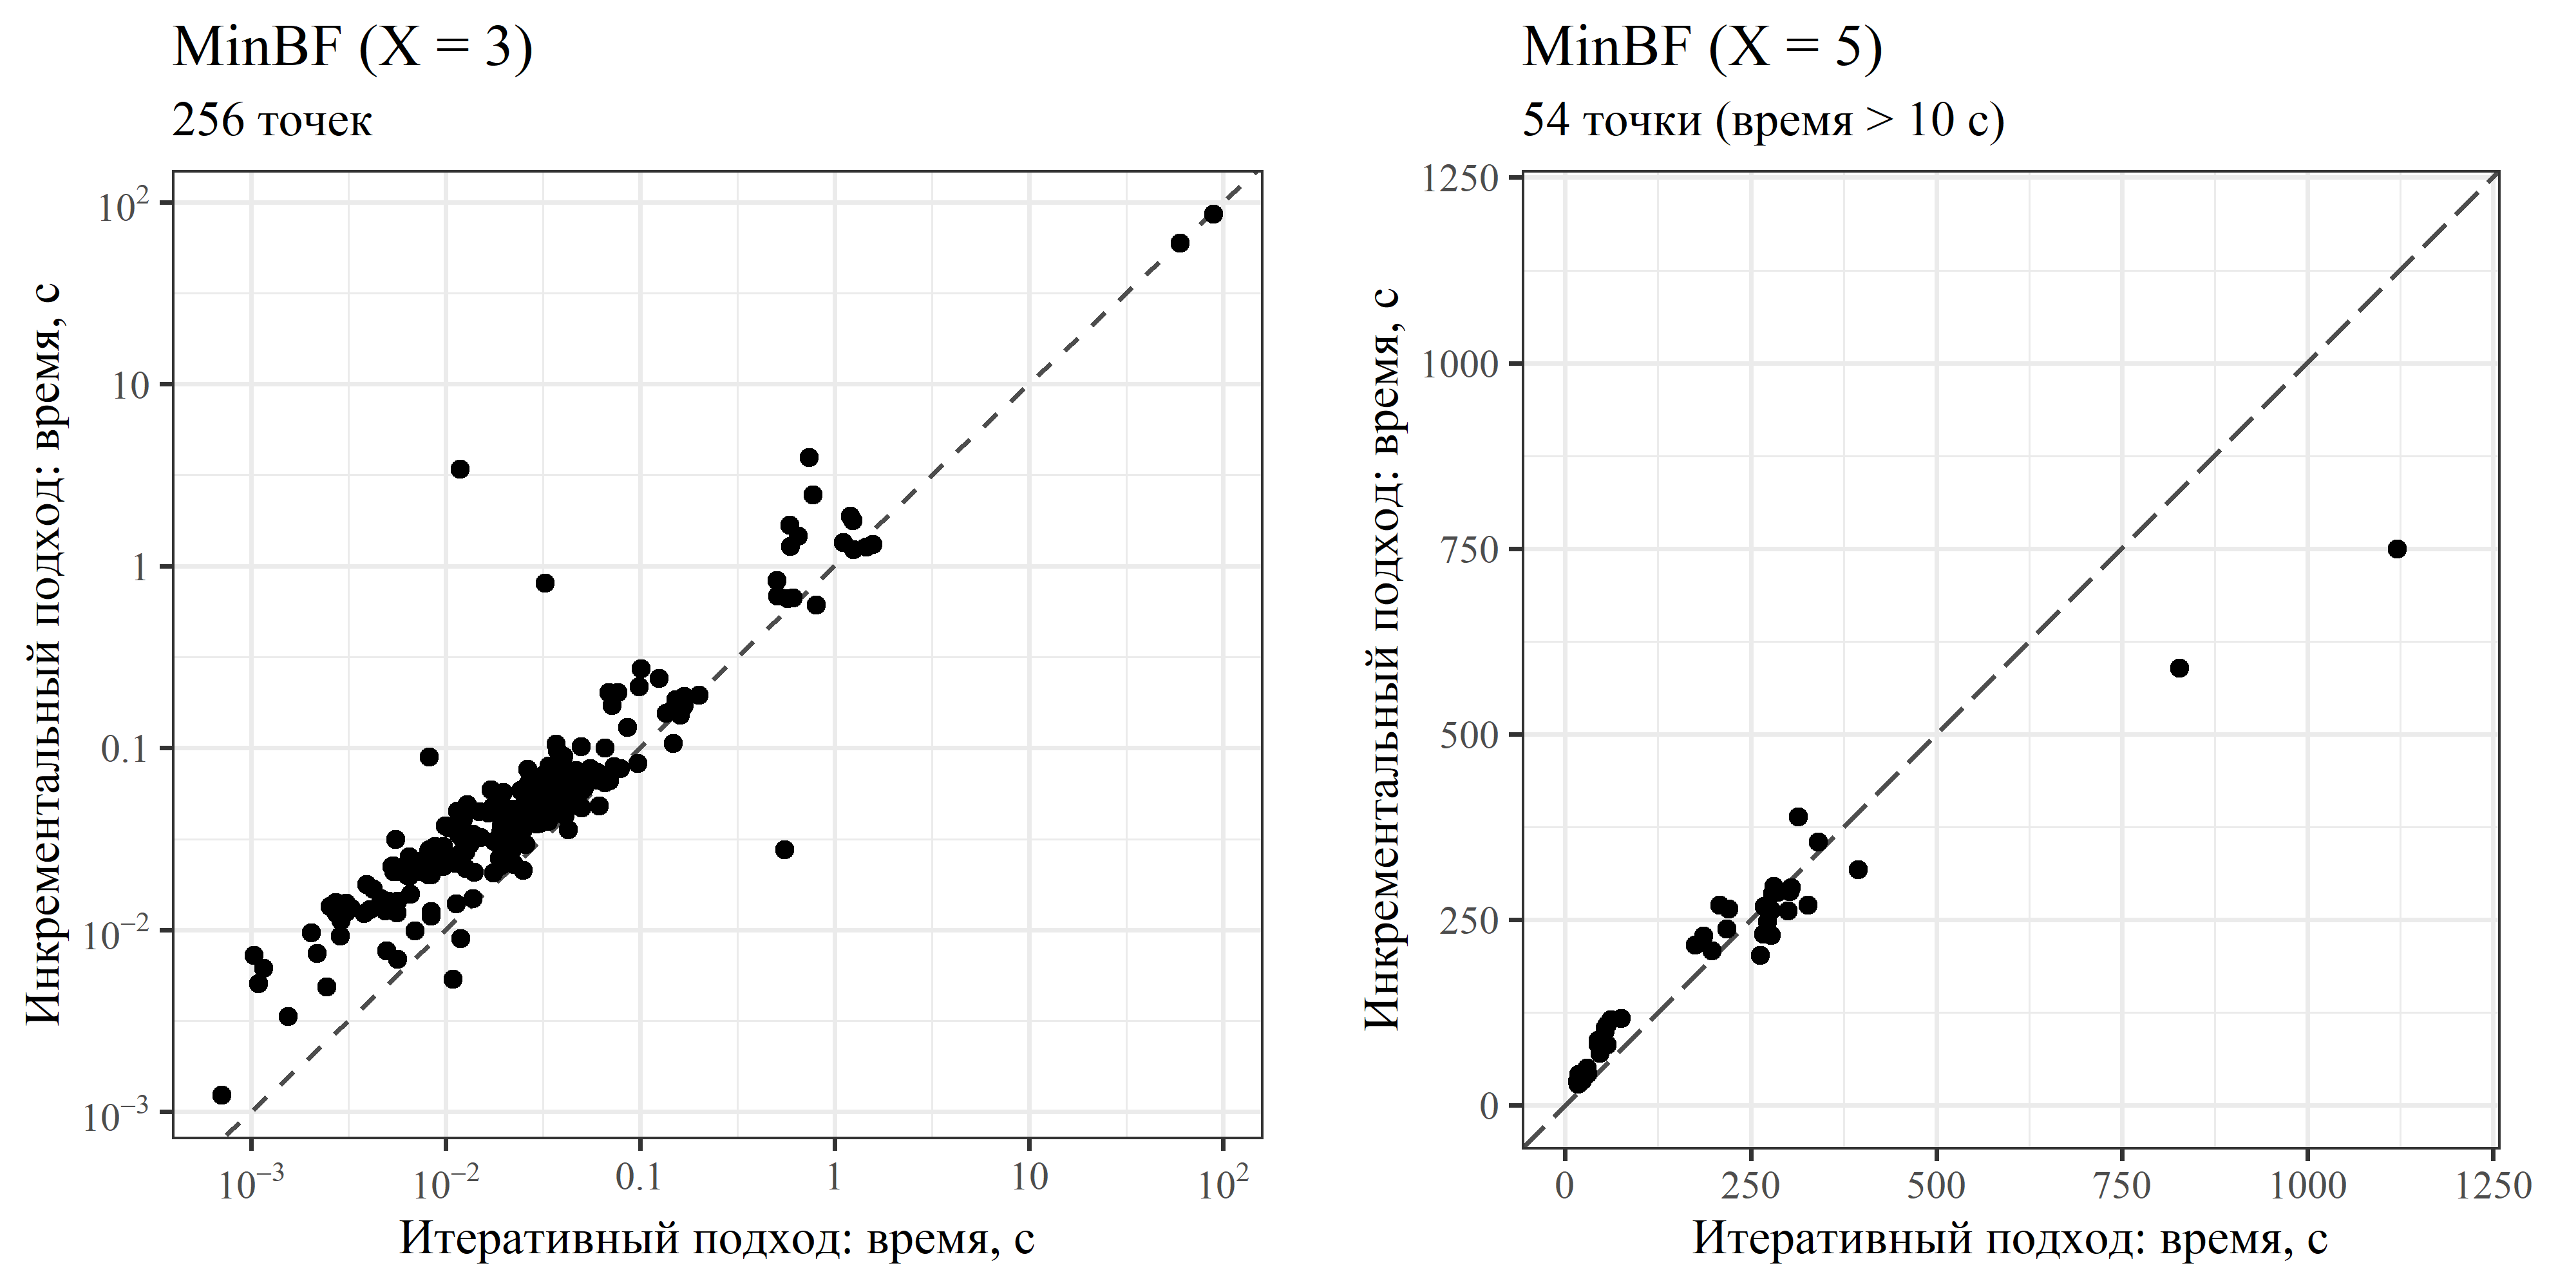
\includegraphics[max width=\linewidth]{minbf.png}
    \caption{Графики сравнения времени работы алгоритма синтеза минимальной булевой формулы (слева \--- от трех переменных, справа \--- от пяти переменных) для двух подходов: итеративный (горизонтальная ось) и инкрементальный (вертикальная ось). Время работы указано в секундах (слева \--- на логарифмической шкале). Каждая точка на графике соответствует булевой функции. На правом графике показаны только точки со временем работы, превышающим 10 секунд.}
    \label{fig:minbf}
\end{figure}

Можно заметить, что большинство минимальных формул для функций от трех переменных были найдены менее, чем за одну секунду \--- сравнение на таких масштабах времени в контексте решения NP-трудных задач не является целесообразным. Поэтому были проведен дополнительный набор экспериментов на данных большей размерности и более «сложных» булевых функциях \--- от $X = 5$ переменных. Результаты приведены на \emph{Рис. 1} (справа), где показаны только точки со временем работы, превышающим 10 секунд (всего 54 точки). Данный график \--- а именно, точки в правой части графика под базовой линией \--- позволяет судить о том, что инкрементальный подход действительно обеспечивает лучшую производительность в рассмотренной задаче синтеза минимальной булевой формулы.



\section{Задача проверки эквивалентности булевых схем}
\label{sub:lec}

Задача проверки эквивалентности булевых схем (Logical Equivalence Checking \--- LEC) является одной из ключевых комбинаторных проблем в автоматизации проектирования электроники.
В этом разделе даны основные понятия о LEC, которые будут использованы в дальнейшем.

Рассмотрим две булевы схемы $S_f$, $S_h$, определяющие функции $f, h: \{0,1\}^n \to \{0,1\}^m$.
Задача LEC заключается в том, чтобы определить, являются ли две заданные схемы эквивалетными, то есть обладают одинаковыми выходами на всех возможных входах, что выражается в том, что соответствующие функции поточечно равны, $f \cong h$.
Задача LEC может быть сведена к задаче выполнимости булевых формул (SAT), ниже это показано на примерах.

\begin{figure}[ht]
    \centering
    \subfile{tex/tikz-glued}
    \caption{Склеенная схема $S_{f \glue h}$, построенная с использованием одного и того же набора входов для двух схем $S_f$ и $S_h$}
    \label{fig:glued}
\end{figure}

Используя $S_f$ и $S_h$, построим новую схему, обозначаемую $S_{f \glue h}$ (см. Рисунок~\ref{fig:glued}), которая получается из $S_f$ и $S_h$ путем \enquote{склейки} вместе входных вершин \--- обозначим её $S_{f \glue h}$.
Она имеет тот же набор входов $\Vin$ как и $S_f$ и $S_h$, и определяет следующую функцию:
\begin{equation}\label{eq:f-glue-h}
    f \glue h \colon \{0,1\}^n \to \{0,1\}^{2m}
\end{equation}
Обозначим через $\Vout_f$ и $\Vout_h$ множества выходов схем $S_f$, $S_h$, а через $Y_f = \{y_1^f, \dots, y_m^f\}$ и $Y_h = \{y_1^h, \dots, y_m^h\}$ множества переменных, связанных с вершинами из $\Vout_f$ и $\Vout_h$ соответственно, упорядоченные согласно семантике схем.
Теперь рассмотрим формулу $(y_1^f \xor y_1^h) \lor \dots \lor (y_m^f \xor y_m^h)$, которая задает булеву функцию $\mathcal{M} \colon \{0,1\}^{2m} \to \{0,1\}$, называемую \textit{miter}~\cite{brand1983}.
Мы обозначим булеву схему, реализующую функцию $\mathcal{M} \circ (f \glue h)$ как $S_{f \xor h}$ и будем ссылаться на нее как на \textit{miter-схему}.
Рассмотрим формулу
\begin{equation}\label{eq:miter-cnf}
    C_{f\xor h} = C_{f \glue h} \land C(\mathcal{M}) ,
\end{equation}
где $C_{f \glue h}$ \=== шаблонная CNF для функции~\eqref{eq:f-glue-h}, а $C(\mathcal{M})$ выглядит следующим образом:
\begin{align*}
    C(\mathcal{M}) = C(w_1 \equiv (y_1^f \xor y_1^h)) \land \dots \land \\
    \land C(w_m \equiv (y_m^f \xor y_m^h)) \land \\
    \land (w_1 \lor \dots \lor w_m) ,
\end{align*}
где $C(w_j \equiv (y_j^f \xor y_j^h))$, $j\in \{1,\dots,m\}$ \--- CNF-представление булевой функции, заданной формулой $w_j \equiv (y_j^f \xor y_j^h)$.
Из Леммы~\ref{lem1} непосредственно следует, что $S_f$ и $S_h$ эквивалентны тогда и только тогда, когда $C_{f \xor h}$ невыполнима.


\section{Задача генерации тестовых шаблонов для верификации булевых схем}
\label{sub:atpg}

В этом разделе рассматривается задача \textit{автоматической} генерации тестовых шаблонов (Automatic Test Pattern Generation \--- ATPG) для верификации булевых схем.
Сначала вводится понятие модели неисправностей (\textit{fault model}).
Затем формулируется задача генерации шаблонов (ATPG) для комбинационных (\textit{combinational}) булевых схем.
Также упоминается секвенциальная (\textit{sequential}) постановка задачи ATPG для схем с элементами памяти, такими как триггеры (\textit{flip-flops}).
Наконец, кратко рассматриваются классические алгоритмы ATPG, работающие на структуре схемы.
% Представление оставлено кратким, для дальнейшего чтения мы ссылаемся на [JG03].
В~разделе~\ref{sub:sat-atpg} отдельно рассматриваются методы решения задачи ATPG, основанные на сведении к задаче выполнимости (SAT), как наиболее релевантные к текущей работе.

\subsubsection{Модель неисправности Stuck-At}

После производства чипа необходимо проверить его функциональную корректность относительно спецификации схемы на уровне булевых элементов.
Без этой проверки некорректный чип будет доставлен заказчикам, что может привести к неполадкам в конечном продукте. Это, конечно же, недопустимо.
С другой стороны, из-за дефектов материала, вариаций процесса во время производства и~т.\@\:д.\@ возможен широкий диапазон неисправностей.
Но непосредственная проверка всех возможных физических дефектов невозможна.
Поэтому вводится абстракция в виде модели неисправности.
Модель неисправности Stuck-At (SAFM) [BF76] хорошо известна и широко используется на практике.
В этой модели неисправности предполагается, что одна линия застряла на фиксированном значении вместо зависимости от значений входов.
Когда линия застряла на значении~0, это называется неисправностью stuck-at-0 (SA0).
Аналогично, если линия застряла на значении 1, это называется неисправностью stuck-at-1 (SA1).

% TODO: \begin{example}
\textbf{Пример.}
Рассмотрим схему, показанную на рисунке 27.7(a). Когда на линии d вводится неисправность SA0, получается неисправная схема, показанная на рисунке 27.7(b). Выход элемента И отключается, и вход элемента ИЛИ постоянно принимает значение 0.

Помимо SAFM было предложено ряд других моделей неисправностей, например, клеточная модель неисправностей [Fri73], где меняется функция одного элемента, или модель мостовой неисправности [KP80], где предполагается, что две линии устанавливаются в одно значение.
Эти модели неисправностей в основном охватывают статические физические дефекты, такие как обрывы или замыкания.
Динамические эффекты охватываются моделями неисправностей задержки.
В~модели неисправности по задержке пути [Smi85] одна неисправность означает, что изменение значения вдоль пути от входов к выходам в схеме не приходит в течение времени цикла тактового сигнала.
Вместо путей модель неисправности задержки на входах элементов [HRVD77, SB77] учитывает задержку в элементах.

Далее рассматривается только SAFM из-за его высокой значимости в практических применениях.
Эту значимость можно объяснить двумя наблюдениями: количество неисправностей имеет порядок размера схемы, и моделирование неисправностей в SAFM относительно просто, то есть для статической модели неисправностей вычислительная сложность генерации тестовых шаблонов ниже по сравнению с динамическими моделями неисправностей.

\subsubsection{Комбинационный ATPG}

Автоматическая генерация тестовых шаблонов (ATPG) \--- это задача определения всех набора тестовых шаблонов для заданной схемы с учетом модели неисправностей.
Тестовый шаблон для конкретной неисправности \--- это назначение на основные входы схемы, которое приводит к различным выходным значениям в зависимости от наличия неисправности.
Вычисление булевой разности между бездефектной и неисправной схемами дает все тестовые шаблоны для конкретной неисправности.
Эта конструкция аналогична схеме \textit{miter}~\cite{brand1983}, поскольку ее можно использовать для проверки эквивалентности комбинационных схем.

% TODO: \begin{example}
\textbf{Пример.}
Снова рассмотрим неисправность SA0 в схеме на рисунке 27.7.
Назначение входов $a = 1$, $b = 1$, $c = 1$ приводит к значению выхода $f = 1$ для корректной схемы и к значению выхода $f = 0$ в случае наличия неисправности.
Поэтому это назначение входов является тестовым шаблоном для неисправности SA0 на линии~$d$.
Конструкция для вычисления булевой разности бездефектной и неисправной схем показана на рисунке 27.8.

Когда тестовый шаблон существует для конкретной неисправности, эта неисправность классифицируется как \textit{тестируемая} (\textit{testable}).
Если тестовый шаблон отсутствует, неисправность называется \textit{избыточной} (\textit{redundant}).
Проблема классификации неисправности как тестируемой или избыточной является NP-полной.
Задача ATPG заключается в классификации всех неисправностей и создании набора тестовых шаблонов, содержащего хотя бы один тестовый шаблон для каждой испытуемой неисправности.

% TODO: \subsubsection{Секвенциальный ATPG}

Генерация тестовых шаблонов для схем, содержащих элементы состояния (памяти), такие как триггеры (\textit{flip-flops}), вычислительно более сложна, потому что элементы памяти не могут быть непосредственно установлены в определенное значение.
Вместо этого поведение схемы во времени должно рассматриваться во время ATPG.
Было предложено ряд инструментов, которые непосредственно решают эту секвенциальную проблему, например, HITEC [NP91].
Но на практике получаемая модель часто слишком сложна для обработки с помощью инструментов ATPG.
Поэтому обычно рассматривается полный режим сканирования для преодоления этой проблемы путем подключения всех элементов состояния в цепочку сканирования [WA73, EW77].
В режиме тестирования цепочка сканирования объединяет все элементы состояния в сдвиговый регистр, в нормальном режиме работы элементы состояния управляются обычной логикой в схеме.
В результате элементы состояния могут рассматриваться как основные входы и выходы для тестирования, и получается комбинационная постановка задачи ATPG, уже рассмотренная выше.

% TODO: \subsubsection{Классические алгоритмы ATPG}

% TODO


\section{Задача булевой выполнимости}
\label{sec:sat}

Задача выполнимости булевых формул (Boolean satisfiability problem \--- SAT) формулируется следующим образом~\cite{handbook-sat}: для произвольной булевой формулы~$\phi(x_1, \dotsc, x_n)$ необходимо определить, существует ли подстановка значений переменных $X_\text{SAT}$, при которой формула становится истинной, то есть, формально, $\exists X_\text{SAT} \in \{0,1\}^n : \phi(X_\text{SAT}) = 1$.
Если такая подстановка существует, то она называется \textit{удовлетворяющей} (\textit{satisfying assignment}; также используются термины \textit{модель} и \textit{интерпретация}), а формула~$\phi$ называется \textit{выполнимой} (\textit{SATisfiable}).
В~противном случае, если удовлетворяющая подстановка не существует, $\phi$~называется \textit{невыполнимой} (\textit{UNSATisfiable}).

Задача SAT является первой задачей, для которой была доказана NP-полнота~\cite{cook}.
\todo{Описание универсальности задачи SAT}

% \subsection{Базовые определения}
% \label{sub:sat-definitions}

% \todo{Литерал, дизъюнкция, конъюнкция, КНФ, ДНФ}

Если булева формула $\phi$ представлена в конъюктивной нормальной форме (КНФ), то соответствующую задачу называют CNF-SAT.
Любая булева формула может быть преобразована в эквивалентную КНФ, однако при этом размер формулы может увеличиться экспоненциально, например:
\[
    \text{$n$ конъюнкций}
    \left\{
    \begin{aligned}
        & (x_1 \land y_1) \lor \\
        & (x_2 \land y_2) \lor \\
        & ~\dots \\
        & (x_n \land y_n)
    \end{aligned}
    \right.
    \quad
    \xRightarrow{\text{КНФ~}}
    \quad
    \left.
    \begin{aligned}
        & (x_1 \lor x_2 \lor \dotsb \lor x_n) \land \\
        & (y_1 \lor x_2 \lor \dotsb \lor x_n) \land \\
        & ~\dotsb \\
        & (y_1 \lor y_2 \lor \dotsb \lor y_n)
    \end{aligned}
    \right\}
    \text{$2^n$ дизъюнкций}
\]
С помощью преобразований Цейтина~\cite{tseitin1970} возможно привести любую булеву формулу в КНФ \--- с сохранением выполнимости (\textit{equisatisfiable CNF}), но с добавлением новых переменных (\textit{auxiliary variable}) \--- при этом размер формулы увеличится лишь линейно.
В данной работе подразумевается, что все булевы выражения, кодирующие задаваемые ограничения, подвергаются либо эквивалентным логическим преобразованиям, либо преобразованиям Цейтина, то есть по итогу представляются в виде КНФ.


\section{Основные алгоритмы решения SAT}

С учетом сказанного в предыдущем разделе, везде далее под задачей о булевой выполнимости (она же SAT) в распознавательном варианте понимается задача распознавания выполнимости произвольной булевой формулы в КНФ. SAT является исторически первой NP-полной задачей. Данный факт был установлен С.А. Куком (без привлечения точного определения NP-полноты) в статье {[}\hl{1}{]}, которая является основополагающей работой для структурной теории сложности алгоритмов. Помимо распознавательного варианта далее нас будет интересовать поисковый вариант SAT \--- когда требуется распознать выполнимость КНФ, и в случае ее выполнимости найти произвольный выполняющий набор. Данная задача, соответственно, NP-трудна. Сказанное означает, что в предположении $P \neq NP$, SAT не может быть решена в общем случае за полиномиальное время. При всем этом существует масса разнообразных аргументов в пользу того, что SAT (как и многие другие NP-трудные задачи) не является сложной в большинстве своих частных случаев. Именно этот факт позволяет использовать современные алгоритмы решения SAT в задачах, комбинаторная размерность которых может быть колоссальной. Так, в символьной верификации удается успешно решать SAT в отношении КНФ, включающих миллионы дизъюнктов. Число переменных, встречающихся в таких КНФ, может исчисляться десятками и сотнями тысяч. В настоящем разделе мы кратко коснемся алгоритмов решения SAT, которые могут применяться к обращению функций вида (1)-(2). Существуют два больших класса алгоритмов решения SAT \--- полные и неполные. Неполные алгоритмы плохо подходят или не подходят совсем для решения задач, в которых требуется доказывать невыполнимость (соответственно, например, для символьной верификации). Однако они вполне могут использоваться для обращения функций.

В настоящей работе основным вычислительным инструментом являются полные алгоритмы решения SAT. Именно такие алгоритмы позволяют точно решать задачи верификации автоматов и булевых схем, то есть находить решение, если оно существует, либо гарантировать его отсутствие при заданных параметрах, что в том числе позволяет точно решать задачу минимизации.


\subsection{Неполные алгоритмы решения SAT}

Неполные алгоритмы решения SAT не гарантируют ответ SAT/UNSAT за конечное время для произвольной КНФ. Существует целый ряд различных концепций, лежащих в основе таких алгоритмов. Статья {[}\hl{2}{]} представляет собой детальный обзор по данному вопросу, содержащий ключевые ссылки. В дальнейшем нас будут интересовать только те неполные алгоритмы решения SAT, в основе которых лежит идеология локального поиска или (в отдельных случаях) эволюционные стратегии. В таких алгоритмах задача SAT в отношении КНФ $C$ над множеством из $n$ переменных, состоящей из $m$ дизъюнктов, рассматривается в форме задачи максимизации псевдобулевой функции

$f_{C} \colon \left\{ 0,1 \right\}^{n} \to \left\{ 0,1,\ldots,m \right\}$. (9)

Напомним здесь, что псевдобулевой (см, например, {[}\hl{3}{]}) называется любая функция вида

$f \colon \left\{ 0,1 \right\}^{n} \to \mathbf{R}\ .$ (10)

На произвольном наборе $\alpha \in \left\{ 0,1 \right\}^{n}$ значение функции (9) равно числу дизъюнктов в $C$, которые на этом наборе обращаются в 1. Фактически в данном случае мы рассматриваем задачу SAT в оптимизационной постановке, известной как MaxSAT.

Рассматривая $\left\{ 0,1 \right\}^{n}$ в роли пространства поиска, можно ввести на нем \textit{функцию окрестностей} {[}\hl{4}{]} $\aleph:\left\{ 0,1 \right\}^{n} \to 2^{\left\{ 0,1 \right\}^{n}}$. Проще всего для этой цели использовать метрику Хэмминга {[}\hl{5}{]}, в рамках которой для произвольной точки $\alpha \in \left\{ 0,1 \right\}^{n}$ ее окрестность Хэмминга радиуса $r,r \geq 1$, определяется следующим образом:

$\aleph_{r}(\alpha) = \left\{ \alpha^{'} \in \left\{ 0,1 \right\}^{n}:\rho_{H}\left( \alpha,\alpha^{'} \right) \leq r \right\}$. (11)

В (11) через $\rho_{H}(\alpha,\alpha')$ обозначено расстояние Хэмминга между словами $\alpha$ и~$\alpha'$. Чаще всего рассматриваются окрестности радиуса~1. В такой постановке для решения SAT и MaxSAT может использоваться, без преувеличения, огромный арсенал методов локального поиска. Мы проиллюстрируем общую идею, лежащую в основе таких методов, на примере простейшего алгоритма, известного как «Восхождение к вершине» (\enquote{\textit{Hill Climbing}} \--- далее HC) {[}\hl{6}{]}. Опишем вариант HC, применимый для максимизации произвольной псевдобулевой функции вида (10).

\begin{enumerate}
\item
  выбираем (вообще говоря, произвольным образом, например, случайно в соответствии с равномерным распределением на $\left\{ 0,1 \right\}^{n}$) стартовую точку $\alpha_{0} \in \left\{ 0,1 \right\}^{n}$, вычисляем $f\left( \alpha_{0} \right)$; считаем $\alpha_{0}$ текущей точкой, а $f \left( \alpha_{0} \right)$ текущим значением $f$;

\item
  пусть $\alpha \in \left\{ 0,1 \right\}^{n}$ \--- текущая точка;

  обходим в некотором порядке $\aleph_{1}(\alpha)\setminus\left\{ \alpha \right\}$, вычисляя для каждой точки $\alpha'$ из данного множества $f(\alpha')$. Если найдена такая точка $\alpha^{'} \in \aleph_{1}(\alpha) \setminus \left\{ \alpha \right\}$, что $f(\alpha') > f(\alpha)$, перейти на шаг 2, в противном случае перейти на шаг 3;

\item
  $\alpha \gets \alpha'$, $f(\alpha) \gets f(\alpha')$, перейти на шаг 1;

\item
  $\left( \alpha,f(\alpha) \right)$ \--- локальный максимум функции $f$ на $\left\{ 0,1 \right\}^{n}$ (поскольку для любой $\alpha^{'} \in \aleph_{1}(\alpha)\setminus \left\{ \alpha \right\}$ имеет место $f(\alpha') \leq f(\alpha)$); в этом случае алгоритм либо останавливается и выдает в качестве ответа $\left( \alpha, f(\alpha) \right)$, либо запускает некоторую процедуру выхода из локального максимума.
\end{enumerate}

Для выхода из локальных экстремумов можно дополнять приведенный выше базовый алгоритм различными техниками, основанными на эвристических и метаэвристических соображениях. Зачастую, выйдя из точки локального экстремума, можно оказаться в точке с худшим значением $f$. Такого сорта «выпрыгивания» из локальных экстремумов могут осуществляться в процессе поиска неоднократно. В этом случае обычно хранится точка с самым лучшим значением функции $f$, достигнутым за все историю поиска. Такое значение называется \textit{рекордом} (\textit{best known value} \--- BKV). Современные техники выхода из локальных экстремумов позволяют даже при решении весьма трудных задач многократно улучшать рекорд в процессе поиска. Если некоторое количество попыток выхода из локальных экстремумов не дает улучшения текущего рекорда $f^{*}$, достигнутого в точке $\alpha^{*}$, то алгоритм останавливается и выдает в качестве ответа пару $\left( \alpha^{*},f^{*} \right)$.

Предположим, что HC применяется к задаче максимизации произвольной функции вида (9). Легко понять, что даже если дополнить HC какой-либо процедурой выхода из точек локального максимума, это не позволит безошибочно распознавать невыполнимость невыполнимых КНФ. С другой стороны, если рассматривается КНФ с большим числом выполняющих наборов, то HC (даже в самом простом варианте) может случайно натолкнуться на такой набор за приемлемое время. Известный пример данного типа \--- успешное использование HC для решения SAT в отношении КНФ, кодирующих задачу размещения $k$ ферзей на шахматной доске размерности $k \times k$ {[}\hl{7}{]}. Однако, к сожалению, HC и известные его модификации напрямую неприменимы к КНФ, кодирующим обращение интересных с практической точки зрения криптографических функций. Причем это верно даже в отношении КНФ с огромным числом выполняющих наборов \--- например, для КНФ, кодирующих задачи обращения криптографических хеш-функций.

Если некоторый алгоритм локального поиска, решающий задачу максимизации функции вида (9), слишком долго не может улучшить текущий рекорд $\left( \alpha,f_{C}(\alpha) \right)$, где $f_{C}(\alpha) < m$, то данный алгоритм можно остановить с ответом «UNSAT» в отношении КНФ $C$. Этот ответ может оказаться ошибочным. Однако существуют специальные техники рандомизации локального поиска, использование которых позволяет оценивать вероятность ошибки указанного типа и даже снижать эту вероятность за счет выполнения алгоритмом большого числа некоторых случайных шагов. Один из самых известных примеров такого рода \--- алгоритм, предложенный У.~Шёнингом в {[}\hl{8}{]}. Данный алгоритм решает задачу о выполнимости произвольной $k$-КНФ, $k \geq 2$, то есть КНФ, каждый дизъюнкт которой имеет длину~$k$. Алгоритм Шёнинга пытается улучшить значение функции (9), достигнутое в точке $\alpha \in \left\{ 0,1 \right\}^{n}$, за счет случайного выбора и модификации тех дизъюнктов в КНФ $C$, которые обращаются в 0 на наборе $\alpha$. Получаемый в результате процесс интерпретируется в рамках хорошо изученной в теории вероятностей модели случайных блужданий {[}\hl{9}{]}. Как результат, если алгоритм Шёнинга, сделав $O\left( n \cdot \left( 2 - \frac{2}{k} \right)^{n} \right)$ простых случайных действий, не находит выполняющий набор, то вероятность ошибиться, заключив, что $C$~невыполнима, не превосходит $1 - \frac{1}{p(n)}$, где через $p( \cdot )$ обозначен некоторый полином. Очевидно, что если повторение упомянутого выше списка действий, скажем, $n \cdot p(n)$ раз не дает выполняющий набор, то заключение о невыполнимости $C$ будет справедливым с вероятностью, которая близка к $1 - e^{- n}$. Идеи, лежащие в основе алгоритма Шёнинга, позволили для SAT в отношении 3-КНФ построить нетривиальные верхние оценки сложности, которые долгое время оставались лучшими среди аналогичных по смыслу оценок (см. {[}\hl{10}{]}, {[}\hl{11}{]}).

Алгоритмы, в которых базовые схемы локального поиска (например, HC) дополняется различными стратегиями рандомизации, относятся к классу, известному как \textit{Stochastic Local Search methods} (SLS). К большому сожалению, имеющиеся на сегодняшний день SLS-алгоритмы плохо подходят для обращения криптографических функций. Как будет показано далее, лучшие такие алгоритмы позволяют успешно решать задачи криптоанализа лишь весьма простых генераторов ключевого потока.

\subsection{Полные алгоритмы решения SAT}

Алгоритм решения SAT называется полным, если для любой КНФ $C$ он за конечное число шагов выдает верный ответ вида SAT/UNSAT. Как и в ситуации с неполными, для построения полных алгоритмов решения SAT можно использовать множество различных базовых концепций. Так, довольно естественно решать SAT, основываясь на широко применяемой в комбинаторной оптимизации идеологии ветвей, границ и отсечений {[}\hl{12}{]}. Хорошо известна сводимость SAT к задаче 0-1-Целочисленное линейное программирование (0-1-ЦЛП), после осуществления которой можно использовать для решения полученной задачи из семейства 0-1-ЦЛП богатый набор программных средств. Также довольно просто перейти от SAT к задаче поиска решений системы алгебраических уравнений степени не выше 2 над полем $GF(2)$. К таким системам можно применять известный алгоритм Б. Бухбергера (он же «метод баз Грёбнера») {[}\hl{13}{]}, а также специальные техники работы с разреженными квадратичными системами над $GF(2)$ (см., например, {[}\hl{14}{]}, {[}\hl{15}{]}).

Многие авторы сходятся во мнении, что лучших результатов в решении трудных вариантов SAT из целого ряда областей, среди которых символьная верификация и криптоанализ, удается добиться за счет использования алгоритмов, относящихся к направлению, которое правильнее всего назвать «Вычислительная логика». Ранние алгоритмы из данного класса лежали в основе первых программных реализаций систем автоматического доказательства теорем \textit{(Automated theorem proving, ATP)}. Одним из таких алгоритмов был «метод Девиса-Патнема» (Davis-Putnam method) {[}\hl{16}{]}. Усовершенствованная версия данного алгоритма, известная как DPLL (от фамилий Davis, Putnam, Logemann, Loveland) {[}\hl{17}{]}, до настоящего момента продолжает использоваться в основе высокоэффективных полных SAT-решателей. DPLL представляет собой обход дерева поиска, в рамках которого выход из тупиковых ветвей организован в форме процедуры, называемой \textit{хронологическим бэктрекингом} (\textit{chronological backtracking}) Остановимся подробнее на тех деталях DPLL, которые потребуются нам в дальнейшем.


\subsection{Алгоритм DPLL}

Пусть $C$ \--- произвольная КНФ над множеством переменных $X$. Пусть $S \subset L_{X}$ \--- произвольное множество литералов над переменными из~$X$, которое не содержит контрарных литералов. Пусть $X_{S}$ \=== множество, включающее все те переменные из $X$, литералы над которыми содержатся в $S$ ($X_{S} \subseteq X$). Рассмотрим отображение
$\sigma \colon X_{S} \to \left\{ 0,1 \right\}\ $,
заданное по следующему правилу:
\(
    \sigma\left( x \in X_{S} \right) = \left\{ \begin{array}{r}
    1,\ x \in S\ \ \ \ \  \\
    0,\ \neg x \in S\ .
    \end{array} \right.\
\) (12)

Иными словами, отображение (12) связывает с выбираемыми из $L_{X}$ литералами значения соответствующих переменных: выбор литерала $x$ интерпретируется как присвоение переменной $x$ значения 1, выбор же $\neg x$, соответствует принятию $x$ значения 0. Множество $S$ будем называть списком литералов, выбранных из $L_{X}$. Теперь опишем собственно алгоритм DPLL.

На начальном шаге список выбранных литералов пуст. Выберем (вообще говоря, произвольный) литерал $l_{1} \in L_{X}$, поместим его в список $S_{1}$ и рассмотрим КНФ $l_{1} \land C$. Удалим из данной КНФ каждый дизъюнкт вида $\left( l_{1} \lor D \right)$, а из каждого дизъюнкта вида $\left( \neg l_{1} \lor D \right)$ удалим литерал $\neg l_{1}$ (здесь через $D$ обозначен произвольный непустой дизъюнкт над $X$). Обозначим результирующую КНФ через $C'$. Будем говорить, что данная КНФ получена из $l_{1} \land C$ в результате применения правила \textit{единичного дизъюнкта} (Unit Propagation rule, UP, {[}\hl{18}{]}) к $C$ и литералу $l_{1}$. Заметим, что если в $C$ содержался дизъюнкт вида $D = \left( \neg l_{1} \lor l' \right)$, то удаление из $D$ литерала $\neg l_{1}$ дает единичный дизъюнкт, состоящий из литерала $l'$. В описанной ситуации литерал $l_{1}$ называют \textit{угаданным}, а про литерал $l'$ говорят, что он был \textit{выведен по правилу единичного дизъюнкта}. К КНФ $C'$ и литералу $l'$ можно снова применить правило единичного дизъюнкта. Если в результате применения UP вывелось несколько литералов, они все ставятся в очередь, после чего к ним и соответствующим КНФ последовательно применяется UP.

Пусть $S_{k} = \left\{ l_{1},\ldots,l_{k} \right\}$ \--- список угаданных литералов. Обозначим через ${\widetilde{S}}_{k}$ список всех литералов, которые были выведены по правилу UP в соответствии с описанной выше процедурой. Пусть $C_{k}$ \=== полученная в результате КНФ. Проанализируем несколько ситуаций, которые могут при этом возникнуть.

\begin{enumerate}
\item
  Пусть ${\widetilde{S}}_{k}$ не содержит контрарных литералов, а $C_{k}$ содержит только единичные дизъюнкты. Тогда $C$ выполнима. Несложно показать, что в этом случае существует выполняющий $C$ набор, в котором значения части (или всех) переменных определяются при помощи отображения (12), применяемого к литералам из $S_{k} \union {\widetilde{S}}_{k}$ .
\item
  Пусть ${\widetilde{S}}_{k}$ не содержит контрарных литералов, а $C_{k}$ содержит дизъюнкты длины не менее 2. Пусть ${\widetilde{C}}_{k}$ \=== КНФ, составленная из этих дизъюнктов, а ${\widetilde{X}}_{k}$ \=== множество переменных, встречающихся в ${\widetilde{C}}_{k}$. Тогда выберем из $L_{{\widetilde{X}}_{k}}$ произвольный литерал $l_{k + 1}$, построим список $S_{k + 1} = S_{k} \union \left\{ l_{k + 1} \right\}$ и применим UP к ${\widetilde{C}}_{k}$ и $l_{k + 1}$.
\item
  Список ${\widetilde{S}}_{k}$ содержит контрарные литералы, то есть пару вида $(l,\neg l)$ для некоторого $l \in L_{X}$. В этой ситуации будем говорить, что список угаданных литералов $S_{k}$ породил конфликт. Сам по себе конфликт еще не означает, что исходная КНФ невыполнима \--- вполне возможно, что она выполнима, но были угаданы такие литералы, что сочетание соответствующих им в смысле отображения (12) значений переменных не встречается ни в одном из выполняющих $C$ наборов.
\end{enumerate}

Пусть $S_{k} = \left\{ l_{1},\ldots,l_{k} \right\}$ \--- список угаданных литералов, такой что после угадывания $l_{k}$ по UP был выведен конфликт. В этой ситуации перейдем от списка $S_{k}$ к списку $S_{k}^{'} = \left\{ l_{1},\ldots,\neg l_{k} \right\}$, помечая литерал $\neg l_{k}$ как «инвертированный». Предположим, что для некоторого $k$ оба списка $S_{k} = \left\{ l_{1},\ldots,l_{k} \right\}$ и $S_{k}^{'} = \left\{ l_{1},\ldots,{\neg l}_{k} \right\}$ порождают конфликты. Пусть $l_{r}$ \=== ближайший предшествующий $l_{k}$ литерал в списке $S_{k}$, который ранее не был инвертирован. Тогда новым списком является $S_{r}^{'} = \left\{ l_{1},\ldots,{\neg l}_{r} \right\}$ (везде здесь предполагалось, что $k,r \geq 2$).

Описанная выше процедура перехода к списку $S_{r}^{'}$ называется хронологическим (обычным) бэктрекингом. Можно заметить, что процесс бэктрегинга соответствует обходу с возвратом бинарного дерева специального вида. Вершинам этого дерева приписаны переменные из $X$. Из произвольной вершины, которой приписана переменная $x$, выходит два ребра, символизирующие литералы $x$ и $\neg x$. Корню данного дерева приписана переменная, над которой берется литерал $l_{1}$. Произвольная ветвь соответствует некоторому списку угаданных литералов. Если такой список порождает конфликт, то соответствующую ветвь назовем тупиковой.

Если для некоторого $k$ списки $S_{k}$ и $S_{k}^{'}$ порождают конфликты, и при этом все литералы, предшествующие $l_{k}$, включая первый, были инвертированы, то каждая ветвь описанного выше дерева поиска является тупиковой. Легко понять, что данный факт означает невыполнимость КНФ $C$. Также в силу всего сказанного выше можно заметить, что число вершин в таком дереве поиска не превосходит $M = 2^{n + 1} - 1$. Отметим, что в реальности это число может быть существенно меньше за счет большого числа литералов, выведенных по UP. Таким образом, применив UP не более $M$ раз, мы либо достигнем ситуации, описанной в пункте 1, и это будет означать, что $C$ выполнима, либо докажем невыполнимость $C$. Все сказанное означает полноту алгоритма DPLL.

\subsection{Концепция CDCL и базирующиеся на ней современные SAT-решатели}

Концепция решения SAT, известная сегодня как Conflict Driven Clause Learning (CDCL), включает в себя ряд важных техник, дополняющих алгоритм DPLL. Первая и главная из них позволяет записывать информацию о конфликте, который возник в процессе обхода дерева поиска, в виде специальным образом построенного дизъюнкта. Такой дизъюнкт называется \textit{конфликтным} (conflict-induced clause). Если $C$ \=== исходная КНФ, а $D$ \=== конфликтный дизъюнкт, то имеет место: $C \to D$, то есть $D$ \=== это логическое следствие (импликация) из~$C$. Соответственно, КНФ~$C$ выполнима тогда и только тогда, когда выполнима КНФ~$C \land D$.

Конфликтные дизъюнкты можно строить различными способами. Приведем простейший пример. Пусть список угаданных литералов $S_{k} = \left\{ l_{1},\ldots,l_{k} \right\}$ породил конфликт в рамках DPLL. Построим следующий конфликтный дизъюнкт: $D = \left( \neg l_{1} \lor \ldots \lor \neg l_{k} \right)$. Данный дизъюнкт запрещает одновременный выбор всех литералов из списка $S_{k}$. Рассмотрим КНФ $C \land D$ ($C$ \=== исходная КНФ). Если мы применим к КНФ $C \land D$ DPLL, используя список угаданных литералов $S_{k - 1} = \left\{ l_{1},\ldots,l_{k - 1} \right\}$, то единичный дизъюнкт $\neg l_{k}$ будет выведен по правилу UP. В этом случае говорят, что вывод литерала $\neg l_{k}$ индуцирован конфликтом. Очень важно, что в данном случае литерал ${\neg l}_{k}$ не угадывается, а выводится по правилу UP на основе информации, полученной в результате анализа конфликта.

Впервые идея использовать конфликтные дизъюнкты для записи информации о тупиковых ветвях в DPLL-поиске была предложена в конференционной статье Ж. Маркеша-Сильвы и К. Сакаллы в 1996 году (см. {[}\hl{19}{]}). В более детальном виде она была представлена этими же авторами в журнальной статье {[}\hl{20}{]}. По сути, именно в этих двух работах были заложены основы концепции CDCL. Еще одна важная техника, которая была описана в {[}\hl{19}{]},{[}\hl{20}{]}, заключается в использовании для представления процесса решения SAT специальных графов, называемых \textit{графами вывода} (\textit{implication graph}). Граф вывода позволяет эффективно выявлять литералы (причем, что важно, как угаданные, так и выведенные по UP), которые ответственны за рассматриваемый конфликт. Графы вывода очень информативны. Разные способы обхода IG соответствуют различным эвристикам формирования конфликтных дизъюнктов. Некоторые такие эвристики также были приведены в {[}\hl{19}{]},{[}\hl{20}{]}.

Основное концептуальное отличие CDCL~от DPLL заключается в том, что CDCL~использует память для хранения информации о ходе поиска в форме конфликтных дизъюнктов. Это позволяет вместо хронологического бэктрекинга в ряде случаев осуществлять \textit{нехронологический бэктрекинг} (\textit{non-chronological backtracking}), называемый также \textit{бэкджампингом} (backjumping). Бэкджампинг \--- это ситуация, когда после анализа конфликта откат в списке угаданных литералов происходит не к ближайшему (от конфликта) литералу, который не был ранее инвертирован, а к угаданному еще раньше (иногда существенно раньше). Во многих случаях бэкджампинг позволяет эффективно отсекать значительные части дерева поиска, запрещая при помощи конфликтных дизъюнктов последующий поиск в этих областях. Первым SAT-решателем, фактически использующим CDCL, был GRASP {[}\hl{19}{]}.

Следующий шаг был сделан в работах {[}\hl{21}{]},{[}\hl{22}{]}, где были введены еще несколько важных техник, дополняющих базовый CDCL. Так, в {[}\hl{21}{]} был описан механизм выбора порядка угадывания литералов, основанный на их «мере конфликтности». Соответствующая эвристика получила называние VSIDS (Variable State Independent Decaying Sum). Также в {[}\hl{21}{]} была описана весьма эффективная техника итеративного применения правила UP, использующая т.н. \enquote{ленивые} (\textit{lazy}) структуры данных, известные как \textit{watched literals}, применяются в настоящее время в большинстве CDCL SAT-решателей. Еще одно важное достижение {[}\hl{21}{]} \--- экспериментальная аргументация пользы рестартов. В статье {[}\hl{22}{]} было проведено детальное исследование различных способов построения конфликтных дизъюнктов за счет анализа графов вывода. На основе результатов работ {[}\hl{21}{]},{[}\hl{22}{]} был построен решатель zchaff \--- первый по-настоящему высокоэффективный SAT решатель, базирующийся на концепции CDCL. С использованием zchaff еще в 2002 году удавалось решать задачи криптоанализа некоторых поточных шифров существенно быстрее простого перебора.

В 2003 году в работе {[}\hl{23}{]} были описаны общие принципы построения высокоскоростного CDCL SAT-решателя с эффективно модифицируемой архитектурой. Исходный код соответствующего решателя, получившего название minisat, был представлен авторами {[}\hl{23}{]} в открытом доступе. Решатель minisat на протяжении многих лет остается де-факто стандартом программной основы эффективных SAT-решателей как широкого профиля, так и нацеленных на конкретную прикладную область. Еще одной важной частью minisat стали процедуры периодической чистки баз конфликтных дизъюнктов. Здесь следует отметить, что грамотно реализованный CDCL в процессе работы может генерировать огромные массивы конфликтной информации. Чрезмерное количество конфликтных дизъюнктов увеличивает число срабатываний правила UP и, как следствие, приводит к падению эффективности вывода. Соответственно, часть конфликтной информации можно попытаться удалить. Однако неудачное удаление конфликтных дизъюнктов может привести к их повторной генерации. В данном контексте особенно ценны эвристики, которые позволяют удалять большое число слабо релевантных конфликтных дизъюнктов. Первые относительно нетривиальные такие эвристики были предложены в статье {[}\hl{24}{]}.

Алгоритмы решения SAT, основанные на CDCL, оказались весьма удачно приспособленными для применения к ним различных концепций распараллеливания. Основными двумя такими концепциями являются т.н. \textit{Portfolio approach} и \textit{Partitioning approach} (далее соответственно, «портфолио-подход» и «подход на основе разбиений»). Детальное сравнение эффективности этих двух подходов предпринято в диссертации А. Хиваринена {[}\hl{25}{]}.

Портфолио-подход предполагает запуск нескольких копий решателя на исходном пространстве поиска, при этом каждая копия начинает работу, используя некоторый набор значений входных параметров SAT решателя (разным копиям соответствуют различные наборы значений параметров). В процессе работы копии решателей могут обмениваться друг с другом конфликтными дизъюнктами. Для достижения высокой скорости такой обмен обычно организуется через оперативную память вычислительного устройства с использованием технологий многопоточного программирования. Соответствующая техника получила название \textit{clause sharing} (\enquote{обмен конфликтными дизъюнктами}). Одна из первых эффективных реализаций обмена конфликтными дизъюнктами была представлена в {[}\hl{26}{]}.

Подход на основе разбиений \textit{(SAT-partitioning)} предполагает разбиение пространства поиска (т.е. фактически множества $\left\{ 0,1 \right\}^{n}$, где $n -$ число переменных в КНФ) на непересекающиеся подобласти, которые обрабатываются независимо друг от друга. Данный подход позволяет организовать решение SAT в параллельной среде со слабо связанными или даже независимыми рабочими процессами (в частности, в грид-средах). Как будет показано далее, подход на основе разбиений дает хорошие результаты при решении SAT-задач, кодирующих криптоанализ блочных и поточных шифров, поскольку естественным образом ассоциируется с атаками, относящимися к классу «угадывай и определяй» (guess and determine) {[}\hl{27}{]}.

Скажем здесь несколько слов по поводу теоретических аргументов эффективности CDCL. Соответствующие результаты относятся к теории сложности пропозициональных доказательств. В этой области исследуется задача доказательства невыполнимости невыполнимой формулы в КНФ. Пусть $C$ \=== произвольная невыполнимая КНФ и $x_{C}$ \=== двоичное слово, представляющее~$C$ в некоторой «разумной» системе кодирования. Пусть $\Sigma_{U} \subset \left\{ 0,1 \right\}^{*}$ \=== множество слов~$x_{C}$ по всем возможным невыполнимым КНФ~$C$. Пусть $A$ \=== произвольный полный алгоритм решения SAT. Любой такой алгоритм называется также системой пропозиционального доказательства (\textit{Propositional proof system}). Получив на вход~$x_{C}$, алгоритм~$A$ выдает двоичное слово~$s$, которое будем называть $A$\=/доказательством невыполнимости~$C$ (см., например, {[}\hl{28}{]}). Рассмотрим функцию $\omega_{A} \colon \left\{ 0,1 \right\}^{*} \to \left\{ 0,1 \right\}^{*}$, определенную следующим образом. Если слово является $A$\=/доказательством невыполнимости некоторой КНФ $C$, то $\omega_{A}$ сопоставляет этому слову слово $x_{C}$. В противном случае выходом $\omega_{A}$ является двоичный код символа $\varnothing$. Несложно понять, что для одной и той же $C$ могут существовать различные $A -$ доказательства ее невыполнимости (особенно хорошо это видно на примере метода резолюций). С~произвольным $x_{C} \in \Sigma_{U}$ свяжем длину кратчайшего $A$\=/доказательства невыполнимости $C$. Можно заметить, что если для некоторого $A$ функция длины кратчайшего $A$\=/доказательства по всем $x_{C} \in \Sigma_{U}$ растет как полином от~$|x_{C}|$, то $\mathrm{NP} = \mathrm{coNP}$ (см. {[}\hl{29}{]}). Однако для целого ряда алгоритмов несложно указать примеры бесконечных семейств невыполнимых КНФ с полиномиально растущей длиной кратчайшего $A$\=/доказательства на этих КНФ.

Пусть теперь $A$ и $B$ \=== два полных алгоритма решения SAT. Пусть $C$ \=== произвольная формула из $\Sigma_{U}$. Если существует полиномиальный алгоритм, который произвольное $A -$доказательство невыполнимости $C$ преобразует в $B -$доказательство ее невыполнимости, то говорят, что система доказательств $B$ полиномиально моделирует систему доказательств $A$. Если $A$ полиномиально моделирует $B$, а $B$ полиномиально моделирует $A$, то данные системы доказательств называются полиномиально эквивалентными. Если на некотором (бесконечном) семействе противоречий ${\Sigma'}_{U} \subset \Sigma_{U}$ длина кратчайшего $A -$доказательства растет как полином от длины КНФ, а длина кратчайшего $B -$ доказательства как экспонента, то очевидно, что $B$ не может полиномиально моделировать $A$. Если при этом $A$ полиномиально моделирует $B$, то разумно считать систему $A$ мощнее системы $B$.

В серии работ конца 90-х \-- начала 00-х годов были получены результаты, касающиеся сложности доказательств в системах, связанных с методом резолюций {[}\hl{30}{]}. В данном контексте важнейший для нас результат содержится в статьях {[}\hl{31}{]},{[}\hl{32}{]}, где было показано, что «общая резолюция» (general resolution) в ее пропозициональном варианте полиномиально эквивалентна алгоритму CDCL с рестартами. Данный факт, в частности, означает, что CDCL имеет экспоненциальную сложность. Действительно, в работе {[}\hl{33}{]} было установлено, что общая резолюция экспоненциальна на семействе логических противоречий, известных как «формулы Дирихле» (Pigeon Hole Principle formulas, $PHP_{n}^{n + 1}$, {[}\hl{34}{]}). В силу сказанного выше, это означает, что и CDCL будет иметь на $PHP_{n}^{n + 1}$ экспоненциальную сложность. В то же время, CDCL является более мощной системой доказательств, чем DPLL (см. {[}\hl{31}{]},{[}\hl{32}{]},{[}\hl{34}{]}).

% \subsection{Алгоритм CDCL}
% \label{sub:cdcl}

% Conflict-Driven Clause Learning (CDCL) \--- это расширение классического алгоритма DPLL, включающее в себя механизмы анализа конфликтов и вывода новых дизъюнктов.
% Алгоритм CDCL лежит в основе многих современных SAT-решателей благодаря своей эффективности при решении экземпляров задачи SAT.
% Ниже приводится подробное описание алгоритма CDCL, а также псевдокод для наглядности.

% \todo{Описание алгоритма CDCL}

\begin{algorithm}[H]
    \caption{DPLL Algorithm with Conflict Analysis and Clause Learning}
    \DontPrintSemicolon
    \SetKwInput{Input}{Input}
    \SetKwInput{Output}{Output}
    \SetKwFunction{AnalyzeConflict}{AnalyzeConflict}

    \Input{Boolean formula $F$, current assignment $\sigma$}
    \Output{satisfying assignment or indication of unsatisfiability}

    \While{not all variables assigned}{
        Branch on unassigned variable $v$ \;
        \eIf{$F$ becomes unsatisfiable under $\sigma \union \{v\}$}{
            $\beta \gets \AnalyzeConflict{$F, \sigma, v$}$ \;
            $F \gets F \union \{\beta\}$ \;
            Backtrack to previous decision level \;
        }{
            Continue recursive exploration \;
        }
    }
\end{algorithm}


\subsection{SAT-решатели}
\label{sub:sat-solvers}

На практике для решения задачи SAT используются специализированные программные средства \--- SAT-\textit{решатели}.
Несмотря на то, что задача SAT имеет экспоненциальную оценку сложности (при условии, что $P \neq NP$), современные SAT-решатели способны решать формулы с миллионами переменных за обозримое время.
Для выбора наиболее эффективного SAT-решателя можно руководствоваться результатами соревнования SAT~Comptetition~\cite{sat-competition}: среди текущих лидеров можно выделить MapleCOMSPS~\cite{liang-2016}, Cadical~\cite{cadical}, CryptoMiniSat~\cite{cryptominisat}, Glucose~\cite{glucose} и Plingeling~\cite{lingeling-and-friends}, хотя на практике эффективность решателей может значительно отличаться, в зависимости от класса рассматриваемых задач.
В некоторых случаях хорошие результаты также показывает MiniSat~\cite{minisat}, являющийся минимальной реализацией CDCL-решателя (\textit{Conflict-Driven Clause Learning}~\cite{grasp}) и служащий основой для многих других решателей (например, CryptoMiniSat и Glucose).

\todo{Инкрементальность}


\section{Методы сведения задач к SAT}
\label{sub:sat-encodings}

\todo{Пример сведения задачи раскраски графа к SAT -- описание переменных и ограничений. Дополнительно -- оптимизационная постановка задачи.}

\todo{LEC as SAT}

\todo{ATPG as SAT}


\section{Декомпозиционная трудность}
\label{sub:dhardness}

Концепция \textit{лазеек} (\textit{backdoors}) была введена в классической работе~\cite{williams2003}.
В частности, множество переменных~$B$ в произвольной КНФ-формуле~$C$ является \textit{сильной лазейкой} (Strong Backdoor Set \--- SBS) для~$C$ относительно некоторого полиномиального алгоритма~$P$ (называемого вспомогательным решателем (\textit{subsolver})), если формула~$C[\beta/B]$ решается с помощью~$P$ (то есть получается ответ SAT/UNSAT за полиномиальное время) для любого~$\beta \in \{0,1\}^{|B|}$.
Здесь через~$C[\beta/B]$ обозначается формула, полученная подстановкой значений~$\beta$ в переменные из~$B$ в~$C$.
Можно заметить~\cite{ansotegui2008}, что если $B$ \=== некоторый SBS, то сложность~$C$ ограничена сверху значением $\fun{poly}(|C|) \cdot 2^{|B|}$, где $\fun{poly}({\cdot})$ \=== некоторый полином.

В статье~\cite{semenov2021} было предложено использовать полный детерминированный SAT-решатель~$A$ в качестве вспомогательного решателя, вместо традиционного полиномиального алгоритма~$P$.
Для оценки производительности решателя, введём следующие обозначения.
Пусть~$t_A(C)$ обозначает время работы~$A$ на КНФ-формуле~$C$.
Сложность формулы~$C$ относительно множества~$B$ и солвера~$A$ может быть определена следующим образом:
\begin{equation}\label{eq:dhardness}
    \mu_{A,B}(C) = \bigsumclap{\beta \in \{0,1\}^{|B|}} t_A(C[\beta/B])
\end{equation}
Минимальное значение~\eqref{eq:dhardness} по всем возможным множествам~$B \in 2^X$ называется \textit{декомпозиционной трудностью} (\textit{decomposition hardness}) формулы~$C$ относительно алгоритма~$A$.

Как показано в~\cite{semenov2021}, значение~\eqref{eq:dhardness} можно выразить с использованием математического ожидания случайной величины~$\xi_B$, связанной с множеством~$B$, которая задается следующим соотношением:
\begin{equation}\label{eq:dh_mc}
    \mu_{A,B}(C) = 2^{|B|} \cdot \E[\xi_B]
\end{equation}
Для оценки значения~\eqref{eq:dhardness} можно использовать метод Монте-Карло и формулу~\eqref{eq:cheb}.
Это сводит задачу оценки сложности декомпозиции к задаче псевдо-булевой \textit{black-box} оптимизации, которая включает перебор различных множеств~$B$ и оценку сложности~$C$ относительно каждого~$B$ в попытке минимизировать это значение в пространстве~$2^X$.
В~\cite{semenov2021} для этой цели использовались метаэвристические алгоритмы.


\section{Вероятностный подход к оцениванию трудности булевых формул}

Предлагаемые в главе~\ref{ch:partitionings} конструкции для декомпозиции формул, кодирующих трудные примеры LEC, основаны на концепции \textit{декомпозиционной трудности}, предложенной в~\cite{semenov2021}. Данная концепция в свою очередь базируется на понятии \textit{лазейки}, введенном в~\cite{williams2003}.

Пусть рассматривается произвольная формула $C$ в КНФ над множеством переменных~$X$. Для произвольного $B \subseteq X$ через $\left\{ 0,1 \right\}^{|B|}$ обозначается множество всех возможных наборов значений переменных из $B$. Пусть $P -$ некоторый полиномиальный алгоритм, который получает на вход произвольную КНФ, а на выход выдает ответ из следующего множества $\left\{ SAT,UNSAT,INDET \right\}$, ответ INDET соответствует ситуации, когда $P$ не может за отведенное время решить, выполнима ли рассматриваемая КНФ. Если применение алгоритма $P$ к формуле $C$ выдает ответ из множества $\left\{ SAT,UNSAT \right\}$, то будем обозначать данный факт через $C \in \Sigma(P)$. Если же результатом применения $P$ к $C$ является ответ $INDET$, то обозначим данную ситуацию через $C \notin \Sigma(P)$.

Через $C\lbrack\beta/B\rbrack$ обозначим формулу, полученную из $C$ в результате подстановки набора $\beta$ значений переменных из $B$. Тогда множество $B$ называется сильной лазейкой (Strong Backdoor Set, SBS), если для любого $\beta \in \left\{ 0,1 \right\}^{|B|}$ имеет место $C\lbrack\beta/B\rbrack \in \Sigma(P)$.

В статье {[}\hl{Ansotegui2008}{]} было отмечено, что любое SBS $B$, существенно меньшее $X$, дает нетривиальную верхнюю оценку трудности формулы $C$, поскольку существует алгоритм со сложностью $poly\left( |C| \right) \cdot 2^{|B|}$, определяющий выполнимость $C$, для некоторого полинома $poly( \cdot )$.

На основании этой идеи в статье {[}\hl{CP2021}{]} был предложен подход к оцениванию трудности произвольных булевых формул, используя их декомпозиционные представления, называемые также разбиениями (Partitioning {[}\hl{Hyvarinen2011}{]}). Более того, оказалось, что оценивать декомпозиционную трудность можно при помощи вероятностных алгоритмов, традиционно относимых к методу Монте-Карло {[}\hl{MetrUlam1949}{]}. Кратко изложим здесь основную суть данного подхода.

Прежде всего напомним понятие разбиения. Согласно {[}\hl{Hyvarinen2011}{]} разбиение (Paritioning) произвольной КНФ над множеством переменных $X -$ это множество формул $\Pi = \left\{ G_{1},\ldots,G_{s} \right\}$ над $X$, такое что выполнены два следующих требования:

\begin{enumerate}
\def\labelenumi{\arabic{enumi}.}
\item
  для любых $i,j \in \left\{ 1,\ldots,s \right\}:$ $i \neq j$ формула $C \land G_{i} \land G_{j}$ невыполнима;
\item
  формула $C$ выполнима тогда и только тогда, когда выполнима формула $C \land \left( G_{1} \lor \ldots \lor G_{s} \right)$.
\end{enumerate}

Очевидно, что если $\Pi -$ некоторое разбиение, то на задачу о выполнимости $C$, можно смотреть как на семейство аналогичных задач для формул вида $C \land G_{i}$, $i \in \left\{ 1,\ldots,s \right\}$. Для решения последних можно использовать параллельные вычисления. SAT задачи для формул вида $C \land G_{i}$ могут быть существенно проще SAT для $C$: если, например, множество $\Pi -$это множество из $2^{k}$ различных кубов над переменными $B = \left\{ {\widetilde{x}}_{1},\ldots,{\widetilde{x}}_{k} \right\}$.

Если $\Pi -$ некоторое разбиение $C$, то по аналогии с понятием лазейки можно определить трудность формулы $C$ относительно $\Pi$ и некоторого алгоритма $A$ решения SAT. Если рассмотреть в роли $A$ некоторый полный SAT решатель, то иногда удается найти относительно небольшие по размеру разбиения, которые вполне можно использовать для решения трудных индустриальных примеров SAT (в том числе верификационной природы). Таким образом, имеет смысл определить трудность $C$ относительно разбиения $\Pi$ как следующую величину:

\[\mu_{A,\Pi}(C) = \sum_{G \in \Pi}^{}{t_{A}(G \land C)}\]

где через $t_{A}(C)$ обозначено время работы полного SAT решателя $A$ на формуле $C$.

Возникает вопрос, как для конкретного разбиения $\Pi$ вычислить, или хотя бы оценить величину $\mu_{A,\Pi}(C)$ в ситуации, когда $s$ велико ? Именно для этой цели может быть использован метод Монте-Карло.

Зададим на $\Pi$ равномерное распределение, приписав каждому $G_{i}$, $i \in \left\{ 1,\ldots,s \right\}$ вероятность $1/s$ и получив таким способом некоторое пространство элементарных исходов. С каждым $G_{i}$ свяжем значение случайной величины $\xi_{\Pi}:\Pi \to R^{+}$, которое на произвольном $G \in \Pi$ равно $t_{A}(G \land C)$. Пусть $Spec\left( \xi_{\Pi} \right) = \left\{ \xi_{1},\ldots,\xi_{r} \right\} -$ спектр величины $\xi_{\Pi}$, а $P\left( \xi_{\Pi} \right) = \left\{ p_{1},\ldots,p_{r} \right\} -$ закон распределения данной величины. Как показано в {[}\hl{CP2021}{]}, имеет место следующий факт:

\[\mu_{A,\Pi}(C) = s \cdot E\lbrack\xi_{\Pi}\rbrack\]

$E\left\lbrack \xi_{\Pi} \right\rbrack -$ математическое ожидание величины $\xi_{\Pi}$. В соответствии с методом Монте-Карло можно оценить величину $\mu_{A,\Pi}(C)$ через значение $\overline{\xi_{\Pi}} = \frac{1}{N} \cdot \sum_{j = 1}^{N}\xi^{j}$, где $\xi^{j},j = 1\ldots N -$ это независимые наблюдения величины $\xi_{\Pi}$. Использование неравенства Чебышёва {[}\hl{Feller1968}{]} даёт следующее соотношение:

\[\Pr\left\{ (1 - \varepsilon)E\left\lbrack \xi_{\Pi} \right\rbrack \leq \overline{\xi_{\Pi}} \leq (1 + \varepsilon)E\lbrack\xi_{\Pi}\rbrack \right\} \geq 1 - \delta\ \ \ \ \ \ \ \ \ \ \ \ \ \ \ \ \ \ \ (1),\]

справедливое для любых фиксированных $\varepsilon,\delta \in (0,1)$ и натурального числа $N$ (число наблюдений), связанных следующим образом:

\[\delta = \frac{Var(\xi_{\Pi})}{\varepsilon^{2}NE^{2}\left\lbrack \xi_{\Pi} \right\rbrack}\ \ \ \ \ \ \ \ \ \ \ \ \ \ \ \ \ \ \ \ \ \ \ (2)\]

Таким образом, с увеличением $N$ точность оценивания $\mu_{A,\Pi}(C)$ величиной $\overline{\xi_{\Pi}}$ будет возрастать. Следует особо отметить, что не существует полных гарантий точности таких оценок: при большой дисперсии и малом $N$ получаемые оценки могут быть сколь угодно неточны. Тем не менее, можно использовать стандартные статистические аргументы точности получаемых оценок. Один метод такого рода описан в {[}\hl{CP2021}{]} и основан на периодическом увеличении объема выборки $N$ до тех пор, пока не выполнится неравенство
\[
    N \geq \frac{s^{2}\left( \xi_{\Pi} \right)}{\delta\varepsilon^{2}\left( \overline{\xi_{\Pi}} \right)^{2}} (3)
\]
в котором $s^{2}\left( \xi_{\Pi} \right) -$ выборочная дисперсия. Неравенство (3) является статистическим аналогом неравенства
\[
    N \geq \frac{Var\left( \xi_{\Pi} \right)}{\varepsilon^{2}\delta E^{2}\left\lbrack \xi_{\Pi} \right\rbrack}.  (4)
\]

Заметим, что условие (\hl{1}) при фиксированных $\varepsilon,\delta \in (0,1)$ имеет место для любого $N$, для которого выполнено (\hl{4}).

Также возможно построение доверительных интервалов для $\mu_{A,\Pi}(C)$ с использованием Центральной предельной теоремы.

% TODO: translate

% Here $\sigma = \sqrt{\fun{Var}(\xi)}$ stands for a standard deviation, $\gamma$ for a confidence level,
% $\gamma = \Phi(\delta_\gamma)$, where $\Phi(\cdot)$ is the normal cumulative distribution function. It means
% that under the considered assumptions the value
% \[
%     \overline{\xi} = \frac{1}{N} \sum_{j = 1}^{N} \xi^{j}
% \]
% is a good approximation of $\E[\xi]$, when the number of observations $N$ is large enongh. For any given $N$ the quality of this approximation depends on the value of $\fun{Var}(\xi)$. In practice, to estimate $\fun{Var}(\xi)$, an unbiased sample variance is used:
% \[
%     s^2 = \frac{1}{N-1} \sum_{j = 1}^{N} \left( \xi^{j} - \overline{\xi} \right)^2.
% \]
% In this case instead of (2) a following formula is applied [32]
% \[
%     Pr\left\{
%         \card{\frac{1}{N} \sum_{j = 1}^{N} \xi^{j} - \E[\xi]} \leq \frac{t_{\gamma, N-1} \cdot s}{\sqrt{N}} ,
%     \right\}
% \]
% where $t_{\gamma, N-1}$ is a quantile of Student's distribution with $N-1$ degrees of freedom that corresponds to the confidence level $\gamma$.
% If, for example, $\gamma = 0.999$ and $N \geq 10000$, then $t_{\gamma, N-1} \approx 3.29$.

% In our case it is important to note that $N$ can be significantly less than $2^d$.
% It means that the preprocessing stage can be used to estimate the total time required for processing the whole decomposition family $\Delta(C, \tilde{X})$.


% {[}\hl{CP2021}{]} Semenov A., Chivilikhin D., Pavlenko A., Otpuschennikov I., Ulyantsev V.,Ignatiev A. Evaluating the hardness of SAT instances using evolutionary optimization algorithms. Proceedings of 27th International Conference on Principles and Practice of Constraint Programming (CP 2021). Editor: Laurent D. Michel; Article No. 47; pp. 47:1-- 47:18.

% {[}\hl{Williams2003}{]} Williams R., Gomes C. P., Selman B. Backdoors to Typical Case Complexity // Proceedings of the 18th International Joint Conference on Artificial Intelligence. Vol. 3 (IJCAI). San Francisco, CA, USA : Morgan Kaufmann Publishers Inc., 08/09/2003. P. 1173--1178.

% {[}\hl{Ansotegui2008}{]}

% {[}\hl{Hyvarinen2011}{]}

% {[}\hl{MetrUlam1949}{]} Metropolis N., Ulam S. The~Monte Carlo Method. Journal of the American Statistical Association. 1949. Vol. 44. Pp. 335-341.

% {[}\hl{Feller1968}{]} Feller W. Introduction to probability theory and its applications. Vol. 1. Wiley. 1968.

% {[}\hl{Wilks1962}{]} Wilks S. Mathematical Statistics. Wiley. 1962.


% \section{Вероятностные лазейки}
% \label{sub:rho-backdoors}

% \todo{$\rho$-backdoors}


\chapterconclusion

\todo{Завершение обзора}
